\section{Simulation}\label{s:simulation}
We have seen in the previous section how the error \(E(x, \alpha) = x^\alpha - \displaystyle \frac{x^{n+1} }{(1 - \beta)x + \beta}\) changes with increasing values of \(\alpha\). Now, we focus on the entire expression, as stated in theorem \ref{t: MGF_inaccurate}.
\subsection{Practical Issues}
Computing these expressions poses some difficulties. In the first place, we want to compute the moment of fractional order \(\alpha\) for a random variable \(X\). Julia does not have any packages to compute raw moments of such an order, thus these moments will have to be created first. In order to accomplish the desired result, we directly compute \(\int_{-\infty}^{\infty} x^\alpha  f_X(x) dx\). If the support of the random variable is infinite, this integral is often not numerically well defined. Thus, in such cases we use a bounded support \((-1000, 1000)\) which provides a sufficient accurate approximation. What is more, for many fractional orders \(\alpha\) in combination with negative values of \(x\), \(x^\alpha\) is of complex form. To avoid such expressions, given that the distribution is symmetric, we simply integrate the PDF over its non-negative support and factor the final value by 2. In this manner, it is still possible to obtain fractional moments of distributions such as the Normal distribution. If a distribution has a negative support and is not symmetric, it is possible to compute the complex or absolute moment of fractional order, which avoids any numerical issues. This approach, however, lacks interpretability, as the intuition behind absolute and complex moments is harder to grasp. 
\newline
It now remains to compute the fractional moment using the Caputo-Fabrizio MGF. Unfortunately, it is rather difficult to compute the fractional derivative of an MGF expression numerically. The reason is, that programming packages often take (fractional) derivatives on a certain point \(x\) rather than over the entire function. Thus, we simply use the result obtained in theorem \ref{t: MGF_inaccurate}. That is, instead of the moment of order \(\alpha\), the Caputo-Fabrizio MGF computes the moment of order \(n+1\) divided by some variables dependent on \(\alpha\). More explicitly, we compute \(\leftindex_{CF}{M}_X^{(\alpha)}(0) = \displaystyle \int_{-\infty}^{\infty}  \frac{x^{n+1} }{(1 - \beta)x + \beta} f_X(x)\). This integral faces the some problems as the aforementioned integral with \(x^\alpha\). What is more, for specific values of \(x\) and \(\beta\), the denominator tends to go towards zero, which is numerically unstable. Thus, in such cases, we add a rather small \(\epsilon\) in order to avoid this issue.

\subsection{Accuracy Analysis}
For this accuracy analysis we consider different parameter values and orders of \(\alpha\). We set \(\alpha \in [0, 5]\) with steps of 0.01. This yields 500 errors per parameter-configuration, which is a reasonably reliable sample size. When possible, we extend \(\alpha\) to the interval \((-1, 0)\). We consider three distributions, namely the Exponential, Normal and Poisson distribution. This selection allows us to cover both continuous and discrete distributions, distributions with negative and positive supports and symmetric distributions. 
\subsubsection{Exponential Distribution}
First we consider the Exponential distribution with PDF as defined in Appendix \ref{s: app_C}.
The support of the Exponential distribution is \([0, \infty)\), thus the integration process will avoid most numerical issues. Moreover, all relevant moments of the Exponential distribution are based on raw moments, which is precisely the kind of moments we are interested in.
\newline
We obtain the following figure:
\begin{figure}[H]
    \centering
    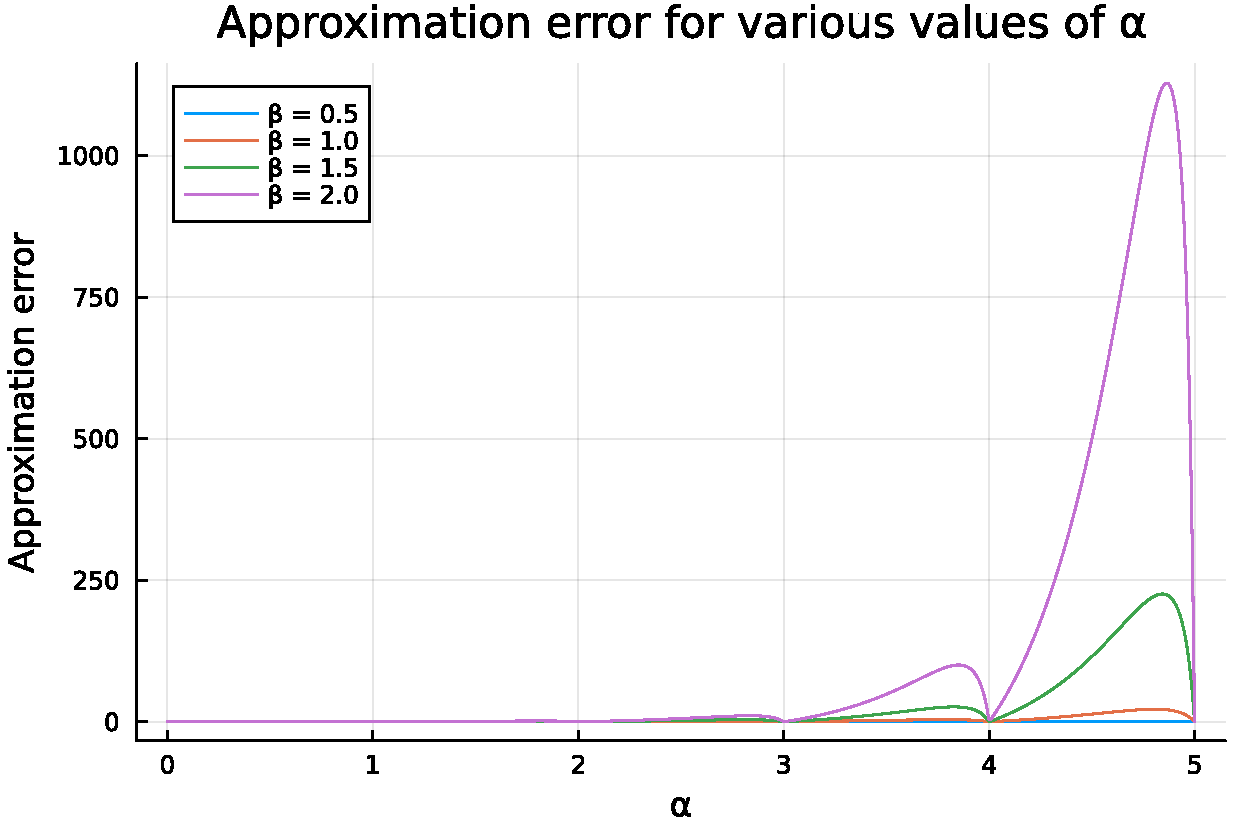
\includegraphics[width=0.8\textwidth]{figures/error_plot_exp.pdf}
    \caption{Approximation error for the Exponential Distribution}
    \label{fig:error_plot_exp}
\end{figure}
From this figure, it is clear that for a greater parameter value \(\beta\) the approximation error increases. Namely, for moments of higher order \((\alpha \geq 3)\), the approximation error increases rapidly. For smaller order \(\alpha\) the approximation errors remain relatively low. In practice, moments of order \(\alpha > 4\) are oftentimes not of interest. Thus, the greatest approximation errors will be avoided.

We obtain the following associated table with some core statistics:
\begin{table}[H]
    \centering
\begin{tabular}{ccccccc}
  \toprule
  \textbf{\(\beta\)} & \textbf{minimum} & \textbf{maximum} & \textbf{mean} & \textbf{standard deviation} & \textbf{skewness} & \textbf{\(c_v\)} \\\midrule
  0.5 & 0.0 & 0.329 & 0.074 & 0.083 & 1.762 & 1.12 \\
  1.0 & 0.0 & 22.119 & 2.907 & 5.612 & 2.314 & 1.93 \\
  1.5 & 0.0 & 225.731 & 25.477 & 54.91 & 2.513 & 2.155 \\
  2.0 & 0.0 & 1128.26 & 115.489 & 265.154 & 2.655 & 2.296 \\\bottomrule
\end{tabular}

\caption{Exponential Distribution - Approximation Error Statistics} 
\label{tab:exp_error}
\end{table}

The results in table \ref{tab:exp_error} align with the conclusions derived in figure \ref{fig:error_plot_exp}. The greater the values of \(\beta\) and \(\alpha\), the greater the (average) approximation error. For all values of \(\beta\), the minimum error is zero, which occurs when \(\alpha \in \mathbb{N}\). An interesting observation is that for \(\beta = 1.5\) the average approximation error exceeds the maximum approximation error for \(\beta = 1.0\). For all values of \(\beta\), the skewness is positive, implying that the distribution of the approximation errors is right-skewed. Thus, clearly the distribution of the errors is not symmetric and therefore certainly not a Normal distribution. In the last column, the Coefficient of Variation has been reported, which has been given by the formula \(\frac{\sigma}{\mu}\), where \(\mu\) and \(\sigma\) denote the sample and sample standard deviation respectively \ref{hendricks1936}. This metric of measurement allows us to objectively compare the variability of the errors of each of the parameter configurations. The lower \(c_v\), the lower the variability and thus the more consistent the dataset. This consistency is something we want to obtain, as it allows us to describe our data with greater confidence. From table \ref{tab:exp_error}, it is clear that the Coefficient of Variation increases as the parameter \(\beta\) increases. For \(\beta = 0.5\) all result are reasonable. The Caputo-Fabrizio MGF in combination with the Exponential(0.5) could still be viable in practice. For Exponential(1), this conclusion may depend on the maximum order of \(\alpha\).

\subsubsection{Normal Distribution}
We now consider \(X\) to be Normally distributed with mean \(\mu\) and standard deviation \(\sigma\), as defined in Appendix \ref{s: app_C}. This distribution is of particular interest as it has two parameters. Thus, we can analyse the differences of effect of both parameters on the approximation error. Therefore, while raw fractional moments of the Normal distribution are not commonly used in practice, we can still obtain valuable insights from this simulation.  The Normal distribution is symmetric with domain \(x \in \mathbb{R}\). So, we integrate the PDF over the interval \((0, 1000)\) to avoid numerical issues.
\newline

We obtain the following figure:
\begin{figure}[H]
    \centering
    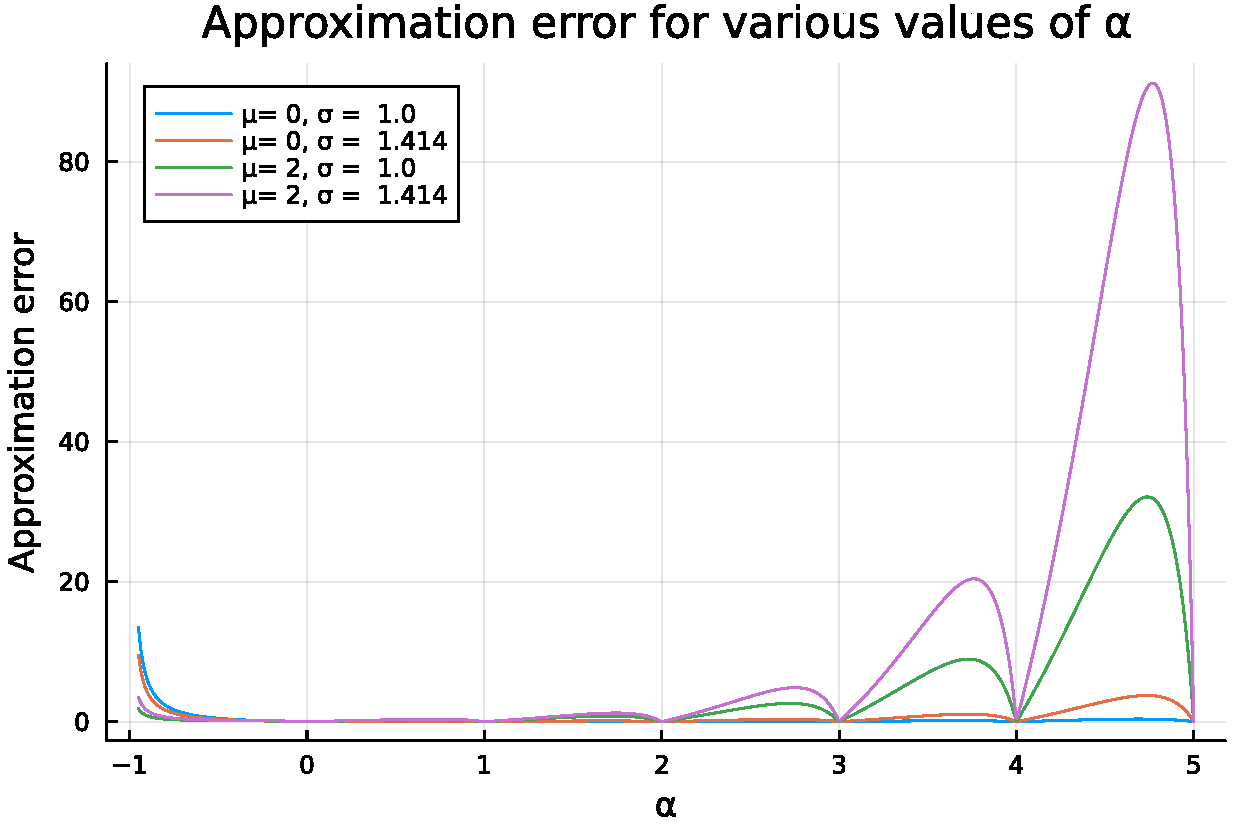
\includegraphics[width=0.8\textwidth]{figures/error_plot_normal.pdf}
    \caption{Approximation error for the Normal Distribution}
    \label{fig:normal_plot_error}
\end{figure}
As illustrated in figure \ref{fig:error_plot_exp}, the approximation error increases with \(\mu\) and \(\sigma\). This result is consitent with the result obtained for the Exponential distribution. However, the magnitude of the errors of the Normal distribution is considerably smaller. Furthermore, the figure also displays the errors for order \(\alpha \in (-0.95, 0)\). These errors tend to attain the same size as errors for order \(\alpha\) near 3. Interestingly, for negative orders of \(\alpha\), the effect of the parameter values seems to reverse. Larger values of \(\mu\) and \(\sigma\) are associated with smaller approximation errors.
\newline 

We obtain the following associated table with some core statistics:
\begin{table}[H]
    \centering
\begin{tabular}{cccccccc}
  \toprule
  \textbf{\(\mu\)} & \textbf{\(\sigma\)} & \textbf{minimum} & \textbf{maximum} & \textbf{mean} & \textbf{standard deviation} & \textbf{skewness} & \textbf{\(c_v\)} \\\midrule
  0.0 & 1.0 & 0.0 & 13.439 & 0.298 & 1.07 & 7.898 & 3.591 \\
  0.0 & 1.414 & 0.0 & 9.505 & 0.7 & 1.141 & 2.824 & 1.629 \\
  2.0 & 1.0 & 0.0 & 32.123 & 4.517 & 8.055 & 2.269 & 1.783 \\
  2.0 & 1.414 & 0.0 & 91.231 & 11.411 & 22.404 & 2.428 & 1.963 \\\bottomrule
\end{tabular}

\caption{Normal Distribution - Approximation Error Statistics} 
\label{tab:normal_error}
\end{table}
The statistics in table \ref{tab:normal_error} support the visuals conclusions drawn from figure \ref{fig:normal_plot_error}. The average of the approximation error for \(\mu = 0\) is acceptable. However, the size of its Coefficient of Variation compared to the other parameter configurations is remarkable. Indeed, configuration \((\mu, \sigma) = (0, 1)\) and configuration \((\mu, \sigma) = (0, \sqrt{2})\) have a rather similar standard deviation, however, but the latter has approximately twice the average error. Except for this case, \(c_v\) again tends to increase as the parameter values increase, suggesting higher variability in approximation errors. Similar to the Exponential distribution, for all parameter-configurations, the distribution of the errors is right-skewed. Thus, the approximation errors of a Normal distribution are not Normally distributed themselves! This result is confirmed in figure \ref{fig:error_histogram}. Even in the histogram of the parameter-configuration with the greatest parameter values, more than 50 percent of the approximation errors cluster around zero, with only a small number of observations falling in the range \((40, 80)\). As before, the average errors and variability for large parameters may be too great to be reliable depending on the context of application.

\begin{figure}[H]
    \centering
    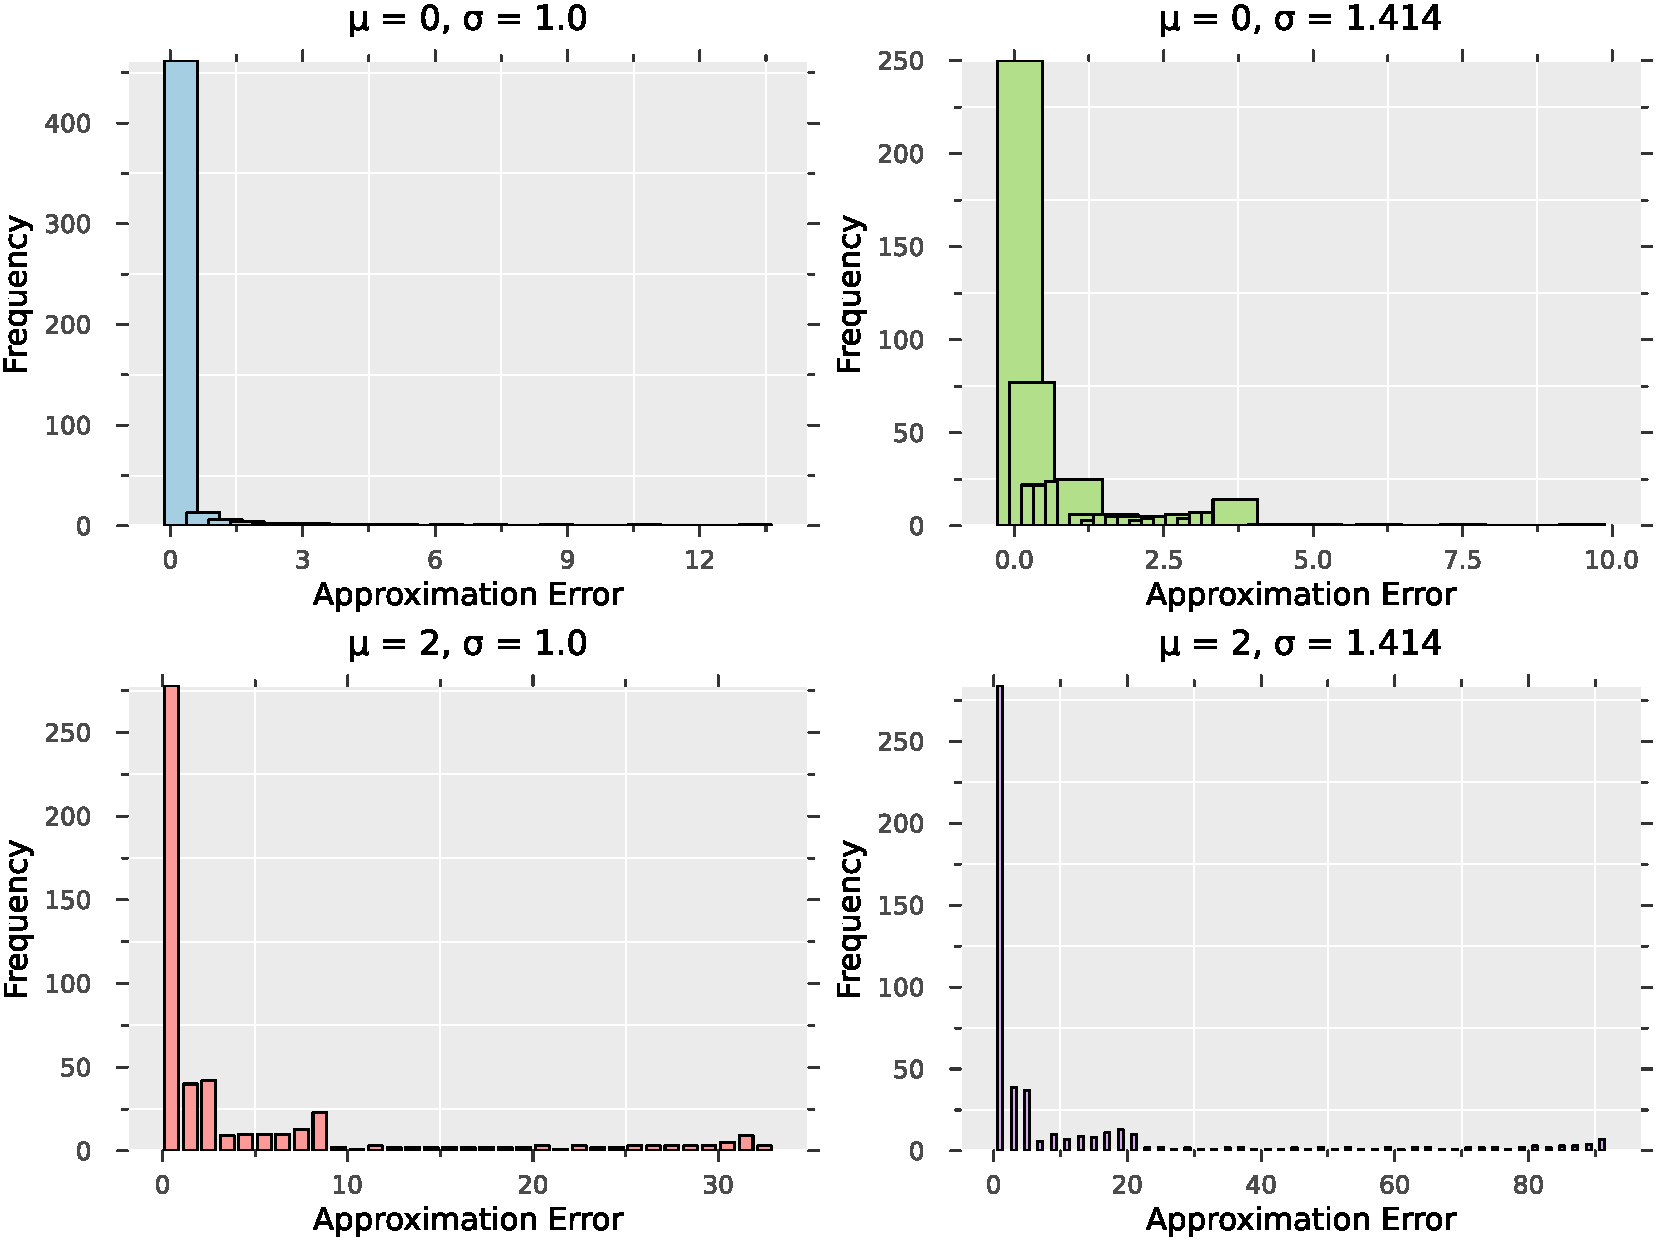
\includegraphics[width=1\textwidth]{figures/error_histogram.pdf}
    \caption{Error Histogram for the Normal Distribution}
    \label{fig:error_histogram}
\end{figure}

\subsubsection{Poisson Distribution}
Finally, we consider a discrete distribution to explore if these results differ from those of the continuous distributions. Specifically, we let \(X \sim Poisson(\lambda)\), with the probaility mass function defined as in Appendix \ref{s: app_C}. The Poisson distribution has positive support and its raw moments are given by: \[\mathbb{E}[X^k] = \sum_{i = 0}^{k} \lambda^i \stirlingii{k}{i}\] with \(k \in \mathbb{N}\) and where \(\{\}\) denotes the Stirling numbers of the second kind (rather similar to the binomial coefficient) \cite{haight1967}. This formula highlights that we cannot consider moment of negative order, as the expression relies on factorials and other combinatorial terms.

We obtain the following figure:
\begin{figure}[H]
    \centering
    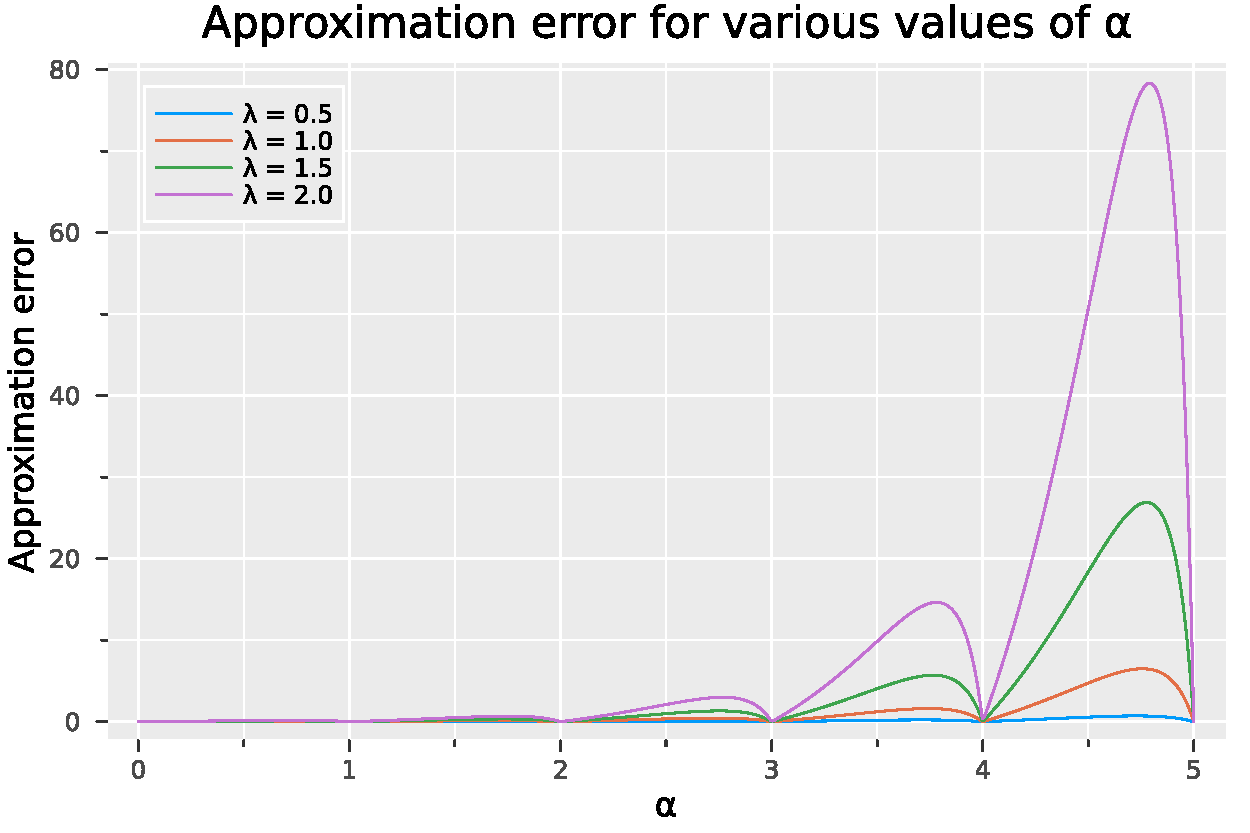
\includegraphics[width=0.8\textwidth]{figures/error_plot_poisson.pdf}
    \caption{Approximation error for the Poisson Distribution}
    \label{fig:poisson_plot_error}
\end{figure}
As shown in figure \ref{fig:poisson_plot_error}, the general trend is consistent with that observed for continuous functions. Larger values of \(\lambda\) lead to greater approximation errors. The magnitude of the errors is comparable to that of the Normal distribution, and increases significantly for \(\alpha \geq 3\).


\begin{table}[H]
    \centering
\begin{tabular}{ccccccc}
  \toprule
  \textbf{\(\lambda\)} & \textbf{minimum} & \textbf{maximum} & \textbf{mean} & \textbf{standard deviation} & \textbf{skewness} & \textbf{\(c_v\)} \\\midrule
  0.5 & 0.0 & 0.715 & 0.128 & 0.191 & 1.915 & 1.494 \\
  1.0 & 0.0 & 6.5 & 1.021 & 1.713 & 2.075 & 1.679 \\
  1.5 & 0.0 & 26.904 & 3.895 & 7.001 & 2.176 & 1.797 \\
  2.0 & 0.0 & 78.34 & 10.687 & 20.143 & 2.251 & 1.885 \\\bottomrule
\end{tabular}

\caption{Poisson Distribution - Approximation Error Statistics} 
\label{tab:poisson_error}
\end{table}
The statistics in table \ref{tab:poisson_error} further support this conclusion
As with previous distributions, the distribution of the errors is right-skewed and the Coefficient of Variation increases as the parameter, \(\lambda\), grows.
For \(\lambda = 0.5\) and \(\lambda = 1.0\), we can still obtain reliable computations. For \(\lambda = 1.5\), the results are still potentially viable, depending on the application and the importance of higher-order fractional moments. In order to minimize its associated standard deviation, one can consider a smaller maximum order of \(\alpha\). In contrast, the configuration \(\lambda = 2.0\) is likely be too unreliable in practice, especially for order \(\alpha > 3\).

\subsection{General results}
Based on the three distributions analysed, we arrive at the following  general conclusions:
\begin{itemize}
    \item As the parameter value of the underlying distribution increase, both the average and maximum approximation error tend to increase.
    \item For all distributions considered, higher parameter values, lead to greater standard deviations in the approximation errors.
    \item Furthermore, the Coefficient of Variationor also increases with larger parameter values, indicating that the standard deviation increases at a higher rate than the mean - a stronger result than the increase in the standard deviation alone.
    \item For all considered distributions and parameter values, the distribution of the approximation errors is right-skewed. Thus, we can conclude that the latter does not follow a Normal, or any other symmetric, distribution.
\end{itemize}
These findings raise important considerations regarding the reliability of the Caputo-Fabrizio MGF in practice. While high parameter values often result in a large Coefficient of Variation, suggesting that the quality of the approximation may behaves inconsistently, figure \ref{fig:error_histogram} offers a different perspective. Namely, in the case of the Normal distribution, at least 50 percent of the errors are clustered around zero. Most importantly, in this section, we are considering a sample of approximation errors of 500 fractional moments. When applying moments of fractional order in practice such as in \cite{hansen2024}, \cite{Mikosc2013} or \cite{gyzl2013}, one usually computes no more than five moments. Considering the latter, metrics such as the standard deviation and Coefficient of Variation may not always be relevant or decisive when evaluating the usability of the Caputo-Fabrizio MGF. Therefore, rejecting a parameter configuration solely based on its high variability may be too strict. In general, as long as the fractional order of the moment remains below 3 or is close to an integer, the Caputo-Fabrizio MGF tends to yield sufficiently accurate results. This supports its viability in practical cases, such as in \cite{hansen2024}, where only fractional moments of relatively low order are of interest.